% Copyright 2006 by Till Tantau
%
% This file may be distributed and/or modified
%
% 1. under the LaTeX Project Public License and/or
% 2. under the GNU Free Documentation License.
%
% See the file doc/generic/pgf/licenses/LICENSE for more details.

\section{Matrices and Alignment}

\label{section-matrices}

\subsection{Overview}

When creating pictures, one often faces the problem of correctly
aligning parts of the picture. For example, you might wish that the
base lines of certain nodes should be on the same line and some
further nodes should be below these nodes with, say, their centers on
a vertical lines. There are different ways of solving such
problems. For example, by making clever use of anchors, nearly all
such alignment problems can be solved. However, this often leads to
complicated code. An often simpler way is to use \emph{matrices},
the use of which is explaied in the current section.

A \tikzname\ matrix is similar to \LaTeX's |{tabular}| or
|{array}| environment, only instead of text each cell contains a
little picture or a node. The sizes of the cells are automatically
adjusted such that they are large enough to contain all the cell
contents.

Matrices are a powerful tool and they need to handled with some care.
For the impatient, note that you \emph{must} end \emph{every} row with
|\\|. In particular, the last row \emph{must} be ended with |\\|.



\subsection{Matrices are Nodes}

Matrices are special in many ways, but for most purposes matrices are
treated like nodes. This means, that you use the |node| path command
to create a matrix and you only use a special option, namely the
|matrix| option, to signal that the node will contain a
matrix. Instead of the usual \TeX-box that makes up the |text| part of
the node's shape, the matrix is used. Thus, in particular, a matrix
can have a shape, this shape can be drawn or filled, it can be used in
a tree, and so on. Also, you can refer to the different anchors of a
matrix. 

\begin{itemize}
  \itemoption{matrix}\opt{|=|\meta{true or false}} This option can be
  passed to a |node| path command. It signals that the node will contain
  a matrix. The default parameter is |true| and should usually be
  omitted.
\begin{codeexample}[]
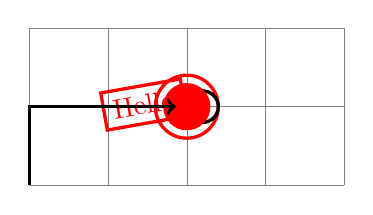
\begin{tikzpicture}
  \draw[help lines] (0,0) grid (4,2);
  \node [matrix,fill=red!20,draw=blue,very thick] (my matrix) at (2,1)
  {
    \draw (0,0)   circle (4mm); & \node[rotate=10] {Hello};        \\
    \draw (0.2,0) circle (2mm); & \fill[red]   (0,0) circle (3mm); \\
  };

  \draw [very thick,->] (0,0) |- (my matrix.west);
\end{tikzpicture}
\end{codeexample}
  The exact syntax of the matrix is explained in the course of this
  section.
  \itemstyle{every matrix}
  This style is used in every matrix. It is empty by default.
\end{itemize}

Even more so than nodes, matrices will often be the only object on a
path. Because of this, there is a special abbreviation for creating matrices:

\begin{command}{\matrix}
  Inside |{tikzpicture}| this is an abbreviation for |\path node[matrix]|.
\end{command}

Even though matrices are nodes, some options do not have the same
effect as for normal nodes:
\begin{enumerate}
\item Rotations and scaling have no effect on a matrix as a whole
  (however, you can still transform the contents of the cells
  normally). Before the matrix is typeset, the rotational and scaling
  part of the transformation matrix is reset.
\item For multi-part shapes you can only set the |text| part of the
  node. 
\item All options starting with |text| such as |text width| have no
  effect.
\end{enumerate}



\subsection{Cell Pictures}

A matrix consists of rows of \emph{cells}. Each row (including the
last one!) is ended by the command |\\|. The character |&| is used
to separate cells. Inside each cell, you must place commands for
drawing a picture, called the \emph{cell picture} in the
following. (However, cell pictures are not enclosed in a complete
|{pgfpicture}| environment, they are a bit more light-weight. The main
difference is that cell pictures cannot have layers.) It is not
necessary to specify beforehand how many rows or columns there are
going to be and if a row contains less cell pictures than another
line, empty cells are automatically added as needed.


\subsubsection{Alignment of Cell Pictures}

For each cell picture a bounding box is computed. These bounding boxes
and the origins of the cell pictures determine how the cells are
aligned. Let us start with the rows: Consider the cell pictures on the first
row. Each has a bounding box and somewhere inside this bounding box
the origin of the cell picture can be found (the origin might even lie
outside the bounding box, but let us ignore this problem for the
moment). The cell pictures are then shifted around such that all
origins lie on the same horizontal line. This may make it necessary to
shift some cell pictures upwards and other downwards, but it can be
done and this yields the vertical alignment of the cell pictures this
row. The top of the row is then given by the top of the ``highest''
cell picture in the row, the bottom of the row is given by the bottom
of the lowest cell picture. (To be more precise, the height of the row
is the maximum $y$-value of any of the bounding boxes and the depth of
the row is the negated minimum $y$-value of the bounding boxes).

\begin{codeexample}[]
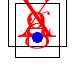
\begin{tikzpicture}
  \tikzstyle{every node}=[draw=black,anchor=base,font=\huge]

  \matrix [draw=red]
  {
    \node {a}; \fill[blue] (0,0) circle (2pt); &
    \node {X}; \fill[blue] (0,0) circle (2pt); &
    \node {g}; \fill[blue] (0,0) circle (2pt); \\
  };
\end{tikzpicture}
\end{codeexample}

Each row is aligned in this fashion: For each row the cell pictures
are vertically aligned such that the origins lie on the same
line. Then the second row is placed below the first row such that the
bottom of the first row touches the top of the second row (unless a
|row sep| is used to add a bit of space). Then the bottom of the
second row touches the top of the third row, and so on. Typically,
each row will have an individual height and depth.

\begin{itemize}
  \itemoption{row sep}|=|\meta{dimension}
  The \meta{dimension} is added between rows as an extra skip. The
  default is |0pt|.
\end{itemize}

\begin{codeexample}[]
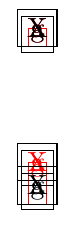
\begin{tikzpicture}
  \tikzstyle{every node}=[draw=black,anchor=base]

  \matrix [draw=red]
  {
    \node {a}; & \node {X}; & \node {g}; \\
    \node {a}; & \node {X}; & \node {g}; \\
  };

  \matrix [row sep=3mm,draw=red] at (0,-2)
  {
    \node {a}; & \node {X}; & \node {g}; \\
    \node {a}; & \node {X}; & \node {g}; \\
  };
\end{tikzpicture}
\end{codeexample}

Let us now have a look at the columns. The rules for how the pictures
on any given column are aligned are very similar to the row
alignment: Consider all cell pictures in the first column. Each is
shifted horizontally such that the origins lie on the same vertical
line. Then, the left end of the column is at the left end of the
bounding box that protrudes furthest to the left. The right end of the
column is at the right end of the bounding box that protrudes furthest
to the left. This fixes the horizontal alignment of the cell pictures
in the first column and the same happens the cell pictures in the
other columns. Then, the right end of the first column touches the
left end of the second column (unless |column sep| is used). The right
end of the second column touches the left end of the third column, and
so on. (Internally, two columns are actually used to achieve the
desired horizontal alignment, but that is only and implementation
detail.) 

\begin{itemize}
  \itemoption{column sep}|=|\meta{dimension}
  The \meta{dimension} is added between columns as an extra skip. The
  default is |0pt|.
\end{itemize}

\begin{codeexample}[]
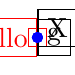
\begin{tikzpicture}
  \tikzstyle{every node}=[draw]
  \matrix [draw=red]
  {
    \node[left]  {Hallo}; \fill[blue] (0,0) circle (2pt); \\
    \node        {X};     \fill[blue] (0,0) circle (2pt); \\
    \node[right] {g};     \fill[blue] (0,0) circle (2pt); \\
  };
\end{tikzpicture}
\end{codeexample}

\begin{codeexample}[]
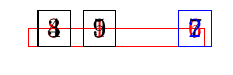
\begin{tikzpicture}
  \tikzstyle{every node}=[draw]
  \matrix [draw=red,column sep=1cm]
  {
    \node {8}; & \node{1}; & \node {6}; \\
    \node {3}; & \node{5}; & \node {7}; \\
    \node {4}; & \node{9}; & \node {2}; \\
  };
\end{tikzpicture}
\end{codeexample}


\subsubsection{Cell Styles and Options}

For following style and option are useful for changing the appearance
of the all cell pictures:
\begin{itemize}
  \itemstyle{every cell} This style is installed at the beginning of
  each cell picture. Note that setting this style to |draw| will
  \emph{not} cause all nodes to be drawn since the |draw| option has
  to be passed to each node individually.

  Inside this style (and inside all cells), the current row and column
  number are accessible via the counters |\pgfmatrixcurrentrow| and
  |\pgfmatrixcurrentcolumn|. 
  \itemoption{cells}|=|\meta{options} This option adds the
  \meta{options} to the style |every cell|. It is just a shorthand for
  |set style={{every cell}+=[|\meta{options}|]}|.
  \itemoption{nodes}|=|\meta{options} This option adds the
  \meta{options} to the style |every node|. It is just a shorthand for
  |set style={{every node}+=[|\meta{options}|]}|.

  The main use of this option is the install some options for the
  nodes \emph{inside} the matrix that should not apply to the matrix
  \emph{itself}. 
\end{itemize}

\begin{codeexample}[]
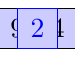
\begin{tikzpicture}
  \matrix [nodes={fill=blue!20,minimum size=5mm}]
  {
    \node {8}; & \node{1}; & \node {6}; \\
    \node {3}; & \node{5}; & \node {7}; \\
    \node {4}; & \node{9}; & \node {2}; \\
  };
\end{tikzpicture}
\end{codeexample}

The next set of styles can be used to change the appearance of certain
rows, columns, or cells. If more than one of these styles is defined,
they are executed in the below order (the |every cell| style is
executed before all of the below).
\begin{itemize}
  \itemstyle{column \meta{number}}
  This style is used for every cell in column \meta{number}.
  \itemstyle{every odd column}
  This style is used for every cell in an odd column.
  \itemstyle{every even column}
  This style is used for every cell in an even column.
  \itemstyle{row \meta{number}}
  This style is used for every cell in row \meta{number}.
  \itemstyle{every odd row}
  This style is used for every cell in an odd row.
  \itemstyle{every even row}
  This style is used for every cell in an even row.
  \itemstyle{row \meta{row number} column \meta{column number}}
  This style is used for the cell in row \meta{row number} and column
  \meta{column number}.
\end{itemize}


\begin{codeexample}[]
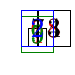
\begin{tikzpicture}
  \tikzstyle{row 1}=[red]
  \tikzstyle{column 2}=[green!50!black]
  \tikzstyle{row 3 column 3}=[blue]
    
  \matrix
  {
    \node {8}; & \node{1}; & \node {6}; \\
    \node {3}; & \node{5}; & \node {7}; \\
    \node {4}; & \node{9}; & \node {2}; \\
  };
\end{tikzpicture}
\end{codeexample}

You can use the |column |\meta{number} option to change the alignment
for different columns.

\begin{codeexample}[]
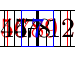
\begin{tikzpicture}
  \tikzstyle{column 1}=[anchor=base west]
  \tikzstyle{column 2}=[anchor=base east]
  \tikzstyle{column 3}=[anchor=base]
  \matrix
  {
    \node {123}; & \node{456}; & \node {789}; \\
    \node {12}; & \node{45}; & \node {78}; \\
    \node {1}; & \node{4}; & \node {7}; \\
  };
\end{tikzpicture}
\end{codeexample}


In many matrices all cell pictures have nearly the same code. For
example, cells typically start with |\node{| and end |};|. The
following options allow you to execute such code in all cells:

\begin{itemize}
  \itemoption{execute at begin cell}|=|\meta{code}
  The code will be executed at the beginning of each cell.
  \itemoption{execute at end cell}|=|\meta{code}
  The code will be executed at the end of each cell.

\begin{codeexample}[]
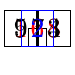
\begin{tikzpicture}
  \tikzstyle{matrix of nodes}=[
    execute at begin cell=\node\bgroup,
    execute at end cell=\egroup;%
  ]
  \matrix [matrix of nodes]
  {
    8 & 1 & 6 \\
    3 & 5 & 7 \\
    4 & 9 & 2 \\
  };
\end{tikzpicture}
\end{codeexample}
\end{itemize}

The |matrix| library defines a number of styles that make use of the
above options.


\subsubsection{Adjusting Column and Row Spacing}

The row-end command |\\| allows you to provide an optional
argument, which must be a dimension. This dimension will be inserted
as an extra row separation between the line being ended and the next
line. Note that this extra skip is in addition to the normal
|row sep|. 
\begin{codeexample}[]
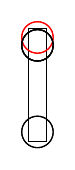
\begin{tikzpicture}
  \matrix [row sep=1mm]
  {
    \draw (0,0) circle (2mm); & \draw (0,0) circle (2mm); \\
    \draw (0,0) circle (2mm); & \draw (0,0) circle (2mm); \\[-1mm]
    \draw (0,0) circle (2mm); & \draw (0,0) circle (2mm); \\[1cm]
    \draw (0,0) circle (2mm); & \draw (0,0) circle (2mm); \\
  };
\end{tikzpicture}
\end{codeexample}

The cell separation character |&| also takes an optional
argument, which must also be a dimension. This causes an extra space
to be inserted between the two columns that are separated by this
character. This optional extra space can only be given the first time
a new column is started (usually in the first row), subsequent usages
of this option in later rows have no effect. Again, this skip is in
addition to |column sep|. Mostly, you will use this skip to slightly
adjust column spacing by adding or removing a few points of space
between columns.
\begin{codeexample}[]
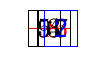
\begin{tikzpicture}
  \tikzstyle{every node}=[draw]
  \matrix [draw=red,column sep=1mm]
  {
    \node {8}; &[2mm] \node{1}; &[-1mm] \node {6}; \\
    \node {3}; &      \node{5}; &       \node {7}; \\
    \node {4}; &      \node{9}; &       \node {2}; \\
  };
\end{tikzpicture}
\end{codeexample}



\subsubsection{Fixed Column and Row Spacing}

Sometimes you may wish to specify a certain distance between the
origins of the cell pictures and you do not care about the size of the
cell pictures themselves. For example, you might wish to have nodes
centered on grid points and the size of the cells is not important.

To achieve this, all you need to do is to make \tikzname\ believe that
the size of each cell is zero, which can be done using the |overlay|
option.

\begin{codeexample}[]
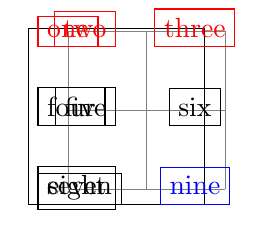
\begin{tikzpicture}
  \tikzstyle{every cell}=[overlay,anchor=mid]
  \draw [help lines] (0,0) grid (2,2);
  
  \matrix [column sep=1cm,row sep=1cm,matrix anchor=one.center] at (0,2)
  {
    \node (one) {one};   & \node{two};   & \node {three}; \\
    \node       {four};  & \node{five};  & \node {six};   \\
    \node       {seven}; & \node{eight}; & \node {nine};  \\
  };
\end{tikzpicture}
\end{codeexample}

As can be seen, this has the disadvantage that the bounding box of the
matrix is no longer correct. A more robust version that does not have
this problem is possible, but not quite trivial to implement.


\subsection{Anchoring a Matrix}

Since matrices are nodes, they can be anchored in the usual fashion
using the |anchor| option. However, there are two ways to influence
this placement further. First, the following option is often useful:

\begin{itemize}
  \itemoption{matrix anchor}|=|\meta{anchor}
  This option has the same effect as |anchor|, but the option applies
  only to the matrix itself, not to the cells inside. If you just say
  |anchor=north| as an option to the matrix node, all nodes inside
  matrix will also have this anchor, unless it is explicitly set
  differently for each node. By comparison, |matrix anchor| sets the
  anchor for the matrix, but for the nodes inside the value of
  |anchor| remain unchanged.

\begin{codeexample}[]
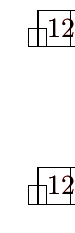
\begin{tikzpicture}
  \matrix [matrix anchor=west] at (0,0)
  {
    \node {123}; \\ % still center anchor
    \node {12}; \\
    \node {1}; \\
  };
  \matrix [anchor=west] at (0,-2)
  {
    \node {123}; \\ % inherited west anchor
    \node {12}; \\
    \node {1}; \\
  };
\end{tikzpicture}
\end{codeexample}
\end{itemize}

The second way to anchor a matrix is to use \emph{an anchor of a node
  inside the matrix}. For this, the |anchor| option has a special
effect when given as an argument to a matrix:

\begin{itemize}
  \itemoption{anchor}|=|\meta{anchor or node.anchor}
  Normally, the argument of this option refers to anchor of the matrix
  node, which is the node than includes all of the stuff of the
  matrix. However, you can also provide an argument of the form
  \meta{node}|.|\meta{anchor} where \meta{node} must be node defined
  inside the matrix and \meta{anchor} is an anchor of this node. In
  this case, the whole matrix is shifted around in such a way that
  this particular anchor of this particular node lies at the |at|
  position of the matrix. The same is true for |matrix anchor|.
\end{itemize}

\begin{codeexample}[]
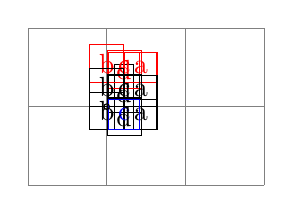
\begin{tikzpicture}
  \draw[help lines] (0,0) grid (3,2);
  \matrix[matrix anchor=inner node.south,anchor=base,row sep=3mm] at (1,1)
  {
    \node {a}; & \node             {b}; & \node {c}; & \node {d}; \\
    \node {a}; & \node(inner node) {b}; & \node {c}; & \node {d}; \\
    \node {a}; & \node             {b}; & \node {c}; & \node {d}; \\
  };
  \draw (inner node.south) circle (1pt);
\end{tikzpicture}
\end{codeexample}



\subsection{Considerations Concerning Active Characters}

Even though \tikzname\ seems to use |&| to separate cells, \pgfname\ actually
uses a different command to separate cells, namely the command
|\pgfmatrixnextcell| and using a normal |&| character will normally
fail. What happens is that, \tikzname\ makes |&| an active character
and then defines this character to be equal to
|\pgfmatrixnextcell|. In most situations this will work 
nicely, but sometimes |&| cannot be made active; for
instance because the matrix is used in an argument of some macro or
the matrix contains nodes that contain normal |{tabular}|
environments. In this case you can use the following option to avoid
having to type |\pgfmatrixnextcell| each time:

\begin{itemize}
  \itemoption{ampersand replacement}|=|\meta{macro name or empty}
  If a macro name is provided, this macro will be defined to be equal
  to |\pgfmatrixnextcell| inside matrices and |&| will not be made
  active. For instance, you could say |ampersand replacement=\&| and
  then use \& to separate columns as in the following example:
\begin{codeexample}[]
\tikz
  \matrix [ampersand replacement=\&]
  {
    \draw (0,0)   circle (4mm); \& \node[rotate=10] {Hello};        \\
    \draw (0.2,0) circle (2mm); \& \fill[red]   (0,0) circle (3mm); \\
  };
\end{codeexample}
\end{itemize}




%%% Local Variables: 
%%% mode: latex
%%% TeX-master: "pgfmanual"
%%% End: 
